
%% vedere come istallare i tool e fare una prima prova con i video presenti sul sito?
%% github

% sezione Conclusioni frame 01

% frame 0
\begin{frame}
	\frametitle{Prerequisiti}
	\framesubtitle{Cosa è bisogna sapere}
	\addtocounter{nframe}{1}

	\begin{itemize}
		\item Buona conoscenza dell’inglese
		\item Nozioni di HTML / CSS / JS
		\item Computer personale o a disposizione per svolgere gli esercizi assegnati
		\item Uso di editor di testo
		\item Uso di editor per programmatori o editor XML
		\item Eseguire comandi da shell
	\end{itemize}

\end{frame}

% frame 0
\begin{frame}
	\frametitle{Strumenti}
	\framesubtitle{Cosa è consigliato usare}
	\addtocounter{nframe}{1}

	\begin{itemize}
		\item Editor di testo professionali (syntax highlighting per XML, workspace)
		\item Editor XML + processore XSLT (normalmente è integrato
		      nell’editor XML)
		\item Navigatore web
		\item Manuali di codifica (Guidelines TEI P5)
		\item Materiale didattico (slide, esempi, esercizi)
	\end{itemize}

\end{frame}

%frame 0
\begin{frame}
	\frametitle{Editor di testo}
	\framesubtitle{Visual Studio Code}
	\addtocounter{nframe}{1}

	\begin{center}
		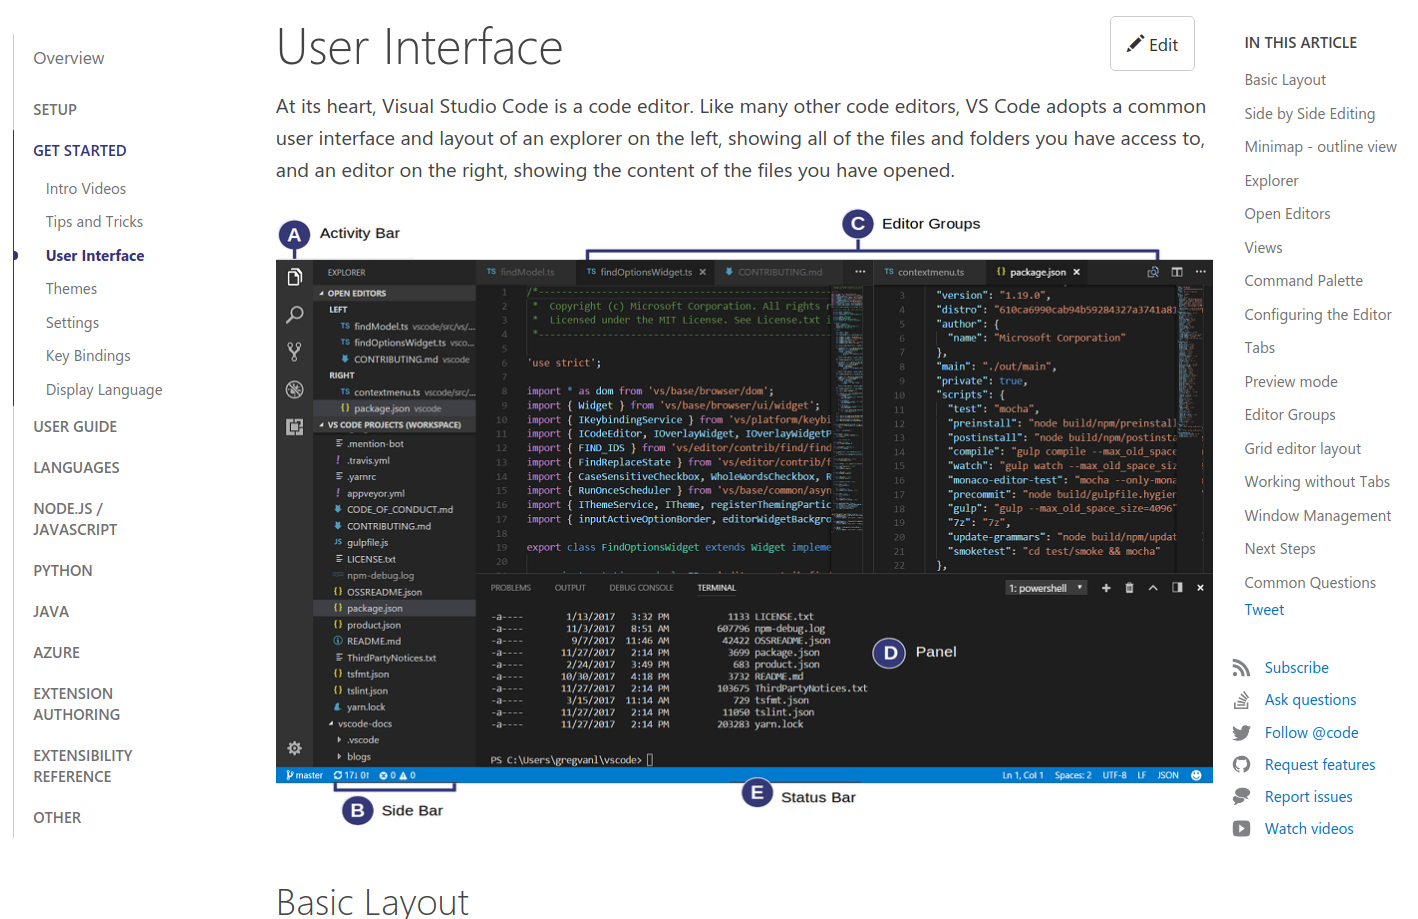
\includegraphics[width=0.9\textwidth]{imgs/VisualCode.png}
	\end{center}

	\href{https://code.visualstudio.com/}{Home page del tool: \url{https://code.visualstudio.com/}}

\end{frame}


%frame 0
\begin{frame}
	\frametitle{Validatore XML}
	\framesubtitle{XMLlint}
	\addtocounter{nframe}{1}

	\begin{center}
		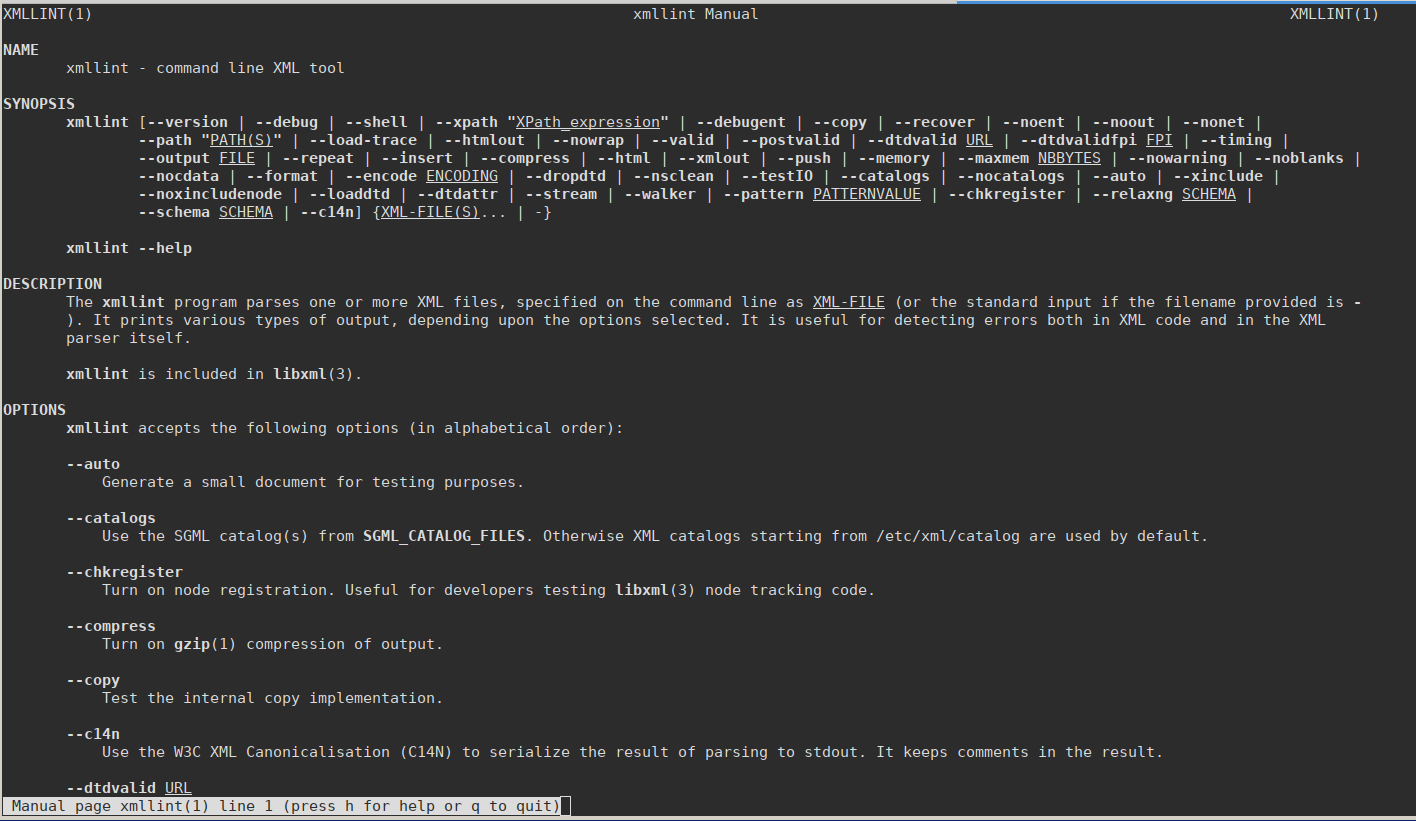
\includegraphics[width=0.9\textwidth]{imgs/XMLLINT.png}
	\end{center}

	\href{http://www.xmlsoft.org/}{Home page del tool: \url{http://www.xmlsoft.org/}}


\end{frame}

% frame 0
\begin{frame}
	\frametitle{Editor XML}
	\framesubtitle{Cosa è consigliato usare}
	\addtocounter{nframe}{1}

	\begin{itemize}
		\item un buon editor open source: XML Copy Editor (http://xmlcopy-editor.sourceforge.net/)
		\item per Mac: XMLSpear, Textmate, Eclipse, IntelliJIDEA
		\item un ottimo editor: Oxygen (http://www.oxygenxml.com/) - multi piattaforma, ma non gratuito (in prova gratuita per un mese)
		\item altri editor: funzioni fondamentali sono la validazione, l’autocompletamento, l’esecuzione di fogli di stile
	\end{itemize}

\end{frame}

\begin{frame}
	\frametitle{Editor XML}
	\framesubtitle{EditiX}
	\addtocounter{nframe}{1}

	\begin{center}
		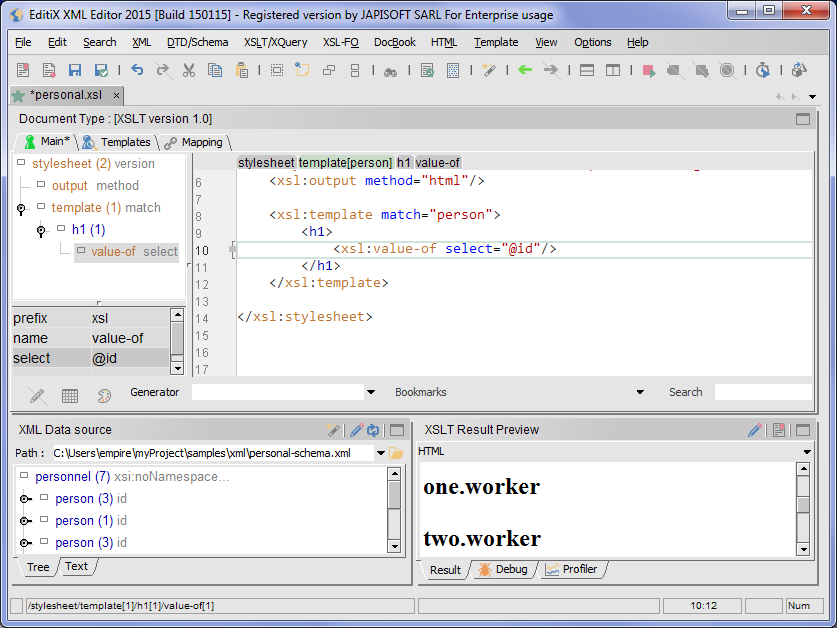
\includegraphics[width=0.8\textwidth]{imgs/maxi2.png}
	\end{center}

	\href{http://www.editix.com}{Home page del tool: \url{http://www.editix.com}}


\end{frame}

% frame 0
\begin{frame}
	\frametitle{Programma d’esame}
	\framesubtitle{Cosa bisogna fare per superare l'esame}
	\addtocounter{nframe}{1}

	\begin{itemize}
		\item Studiare i lucidi delle lezioni
		\item Padroneggiare gli esercizi svolti durante il corso
		\item Studiare i testi indicati dal docente
		\item Studiare i capitoli delle Guidelines TEI che riguardano il corso e il progetto
		\item Realizzare il progetto di codifica concordato con il docente
	\end{itemize}

\end{frame}

% frame 0
\begin{frame}
	\frametitle{Modalità d’esame}
	\framesubtitle{In cosa consiste l'esame}
	\addtocounter{nframe}{1}

	\begin{itemize}
		\item Invio del progetto (obbligatoriamente tramite github)
		\item Colloquio
		      \begin{itemize}
			      \item Discussione del progetto
			      \item Verifica delle conoscenze di base XML, XSD, XSL
			      \item Verifica delle basi teoriche
			      \item Conoscenza di TEI P5 (moduli principali, parti spiegate a lezione, moduli particolari utilizzati nel progetto)
		      \end{itemize}
	\end{itemize}

\end{frame}

% sezione Conclusioni frame 0
\begin{frame}
	\frametitle{Materiale didattico}
	\framesubtitle{Riferimenti per studiare}
	\addtocounter{nframe}{1}

	\begin{block}{Slide}
		\begin{itemize}
			\item Slide delle lezioni corso a.a. 2018-2019
			\item Materiale integrativo fornito dal docente
			\item Repo github del corso \href{https://github.com/angelodel80/corsoCodifica}{\url{https://github.com/angelodel80/corsoCodifica}}
		\end{itemize}
	\end{block}


\end{frame}

\begin{frame}
	\frametitle{Materiale didattico}
	\framesubtitle{Riferimenti per studiare}
	\addtocounter{nframe}{1}

	\begin{block}{Libri}
		\begin{itemize}
			\item Burnard, L. (2014). What is the Text Encoding Initiative? How to add intelligent markup to digital resources. Marseille: OpenEdition Press.
			\item Ciotti, F. (2007). Il testo e l’automa: saggi di teoria e critica computazionale dei testi letterari. Aracne.
			\item Goldberg, K. H. (2010). XML: Visual QuickStart Guide. Pearson Education.
			\item Carey, P., and Vodnik, S. (2014). New Perspectives on XML, Comprehensive. Cengage Learning.			
		\end{itemize}

	\end{block}
\end{frame}

\begin{frame}
	\frametitle{Materiale didattico}
	\framesubtitle{Riferimenti per studiare}
	\addtocounter{nframe}{1}

	\begin{block}{Siti Web}
		\begin{itemize}
			\item \href{https://www.w3.org/XML/}{\url{http://www.tei-c.org/}}
			\item \href{http://teibyexample.org/}{\url{http://teibyexample.org/}}
			\item \href{https://www.w3.org/standards/xml/}{\url{https://www.w3.org/standards/xml/}}
		\end{itemize}

	\end{block}

\end{frame}


